\subsection{Subpaso 1-A: Iniciar estadísticas por pregunta}
	En la configuración de las estadísticas se tiene que seleccionar el 
	inciso \textbf{por pregunta} y la pregunta que desea 
	consultar.
		
	\begin{figure}[hbtp]

	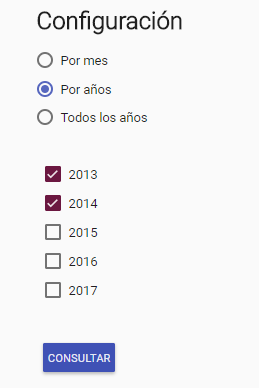
\includegraphics[scale=0.5]{images/Interfaz/IUGS15_configuracioAnos.PNG}
	\caption{Configuración por pregunta }
	\end{figure}
	A continuación se aprieta el botón \textbf{Consultar Pregunta}
	
\subsection{Subpaso 1-B: Muestra de Pregunta}
	Se mostrará la siguiente interfaz con la pregunta elegida:
	\begin{figure}[hbtp]
		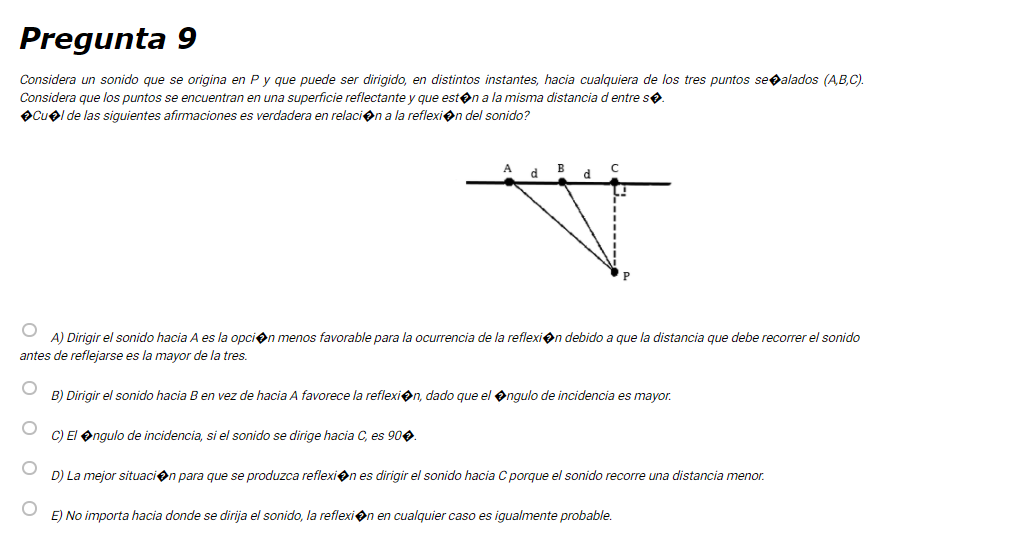
\includegraphics[scale=0.5]{images/Interfaz/IUGS15_estadisticasAnos.PNG}
		\caption{Pregunta}
	\end{figure}	
	
\begin{itemize}
	\item  Las estadísticas que se mostraran son las siguientes:
	\begin{enumerate}
		
		\item Gráfica con los números de la escala para dicha pregunta
		\item Promedio de dificulta de la pregunta
		\begin{figure}[hbtp]
	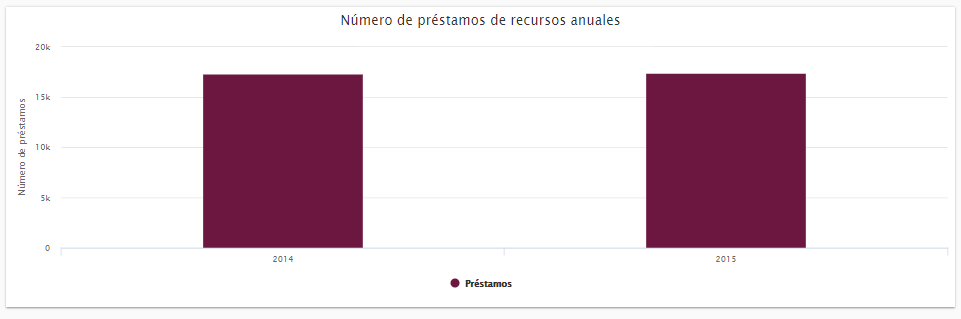
\includegraphics[scale=0.7]{images/Interfaz/IUGS15_recursosAnos.PNG}
	\caption{Gráfica escalas}
	\end{figure}
	


	\end{enumerate}
	
\end{itemize}
\subsection{Subpaso 1-C: Opinión de cada profesor}
Se muestran las opiniones de cada uno de los profesores que opinaron acerca 
de la pregunta propuesta.
\begin{itemize}
	\item Nombre del profesor
	\item Opinión 
\end{itemize}

\begin{figure}[hbtp]
	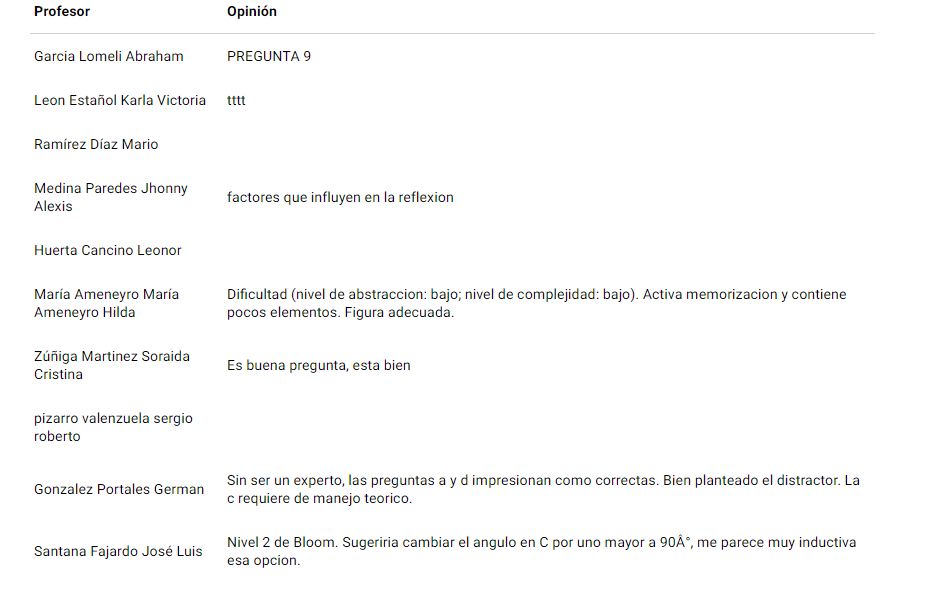
\includegraphics[scale=0.5]{images/Interfaz/IUGS15_opinionPorPregunta.PNG}
	\caption{Opinión de cada profesor por pregunta}
	\end{figure}